\documentclass{article}
\usepackage[utf8x]{inputenc}
\usepackage{latexsym}
\usepackage{amsmath}
\usepackage{float}
\usepackage{graphicx}
\usepackage{booktabs}
\usepackage{url}
\usepackage{subcaption}
\usepackage{hyperref}
\usepackage{booktabs}
\usepackage{adjustbox}

\title{Gender bias in Language from a Natural Language Processing Perspective}
\author{Shawon Ashraf \\ st170090@stud.uni-stuttgart.de}
\date{29 September 2021}



\newcommand\BibTeX{B{\sc ib}\TeX}
%\addbibresource{bib.bib}

\begin{document}

\maketitle

\section*{Introduction}
Language is one of the most powerful and expressive mediums for humans to express their ideas. However it does not stop at being only a tool for communication, language also influences how humans perceive and build their thought process. This inadvertently dictates how humans develop a notion of structure and entities, for example society, class, gender etc. As Ludwig Wittgenstein had famously said that the limits of our languages define the limits of our cognitive boundary. Since language is a necessary prerequisite to describe any entity or class, which in this paper will be human gender, brings the question that if we can think of the social structure with our language and build around it, does the biases and stereotypes, specifically the ones towards gender get into language as well? Or is it that they are intertwined with human cognition and thus get carried over to the language we use for daily communication. Furthermore, for any Natural Language Processing task, language is the source of data, be it written (text corpora) or spoken (as speech signals). So this brings another question into light, if language can get biased from human cognition and the same language is used as a source for NLP applications, how much such biases affect NLP applications and our usage of language in our daily lives? In this paper, we look forward to finding answers for such queries and explore how gender bias is embedded in the ways we use our languages.

\section*{Gender in Language}
% How gender is perceived in language
To begin our discussion, we first need to look at how gender is defined in language in a formal way. As described in \cite{menegatti2017gender}, languages can be categorized \cite{braun2005cognitive} as Genderless Languages (Finnish, Turkish etc.), Natural Gender Languages (English etc.) and Grammatical Gender Languages (German, Italian etc.).

\noindent
\\
The key differentiator in this categorization is how gender is described in the lexical expressions of a language. Genderless languages do not have grammatical gender for nouns or pronouns, rather for words such as Mother, Father, Sister etc. they resort to what is described as "sex-marking". In Natural Gender Languages, pronouns are used to differentiate between genders and nouns can refer to both male and females, e.g. Doctor, Teacher, Nurse etc. Grammatical Gender Languages have their nouns distinguish between male and female entities and often, the female counterpart of a male word is inflicted from the male word. For example, in German, the female for \textit{Lehrer (Teacher)} is \textit{Lehrerin}. Again, the gender of a word is often defined by the surrounding parts of speech, e.g. \textit{Löffel(Spoon)} is masculine and \textit{Gabeln(Fork)} is feminine. To keep our discussion on point we are going to focus solely on the natural use of gender in language with sex-marking instead of grammatically motivated gender since it corresponds to the topic at hand.

\section*{Social View of Gender}
According to \cite{larson2017gender}, gender can be perceived as a social construct in the following ways : 


\begin{figure}[H]
    \centering
    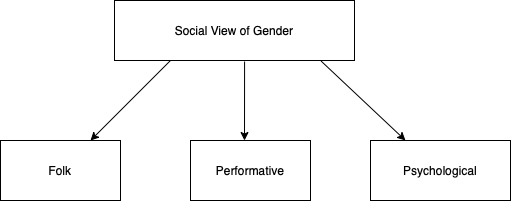
\includegraphics[width=0.8\textwidth]{Gender Social View.png}
    \caption{Gender as a social construct}
    \label{fig:gender_social_view}
\end{figure}

\noindent
The folk refers to common beliefs regarding gender orientation in a society. These views can be motivated by age old traditions or religion or both. The folk point of view regarding gender can be limiting depending on the culture and other factors and also a big contributor to our topic discussion which is bias towards a specific gender. We will discuss this effect in a later section of the paper. \\


\noindent
The performative view towards gender is based on what roles society assigns to a gender and expects people to conform to. These roles can be motivated by the folk point of view but the society can also have its own. For example in matriarchal societies in many Asian countries, women are regarded as the key figures and they have the final say when it comes to taking decisions. Likewise in a different form of society, the norms will expect that some tasks or occupation to be handles only by the male members while their female counterparts should maintain the households. We can also say that this a more constrained and imposed view of gender. \\

\noindent
The psychological view on the other hand is not constrained by society or traditional norms. This view rather focuses on the characteristics(such as self-reliance, independence, loyalty, sympathy etc.) of the existing gender and tries to find a cluster based on these characteristics. \\

\noindent
However, \cite{larson2017gender} also suggest that devising a hierarchy like the one described here is an open ended task and is much more dependent on the research question on what someone expects to do with gender. 

\section*{Gender Bias in Linguistic Processes}
How linguistic components affect cognition and introduce bias towards genders

\section{Bias in Data}
Source of bias in data, how it's connected to cognitive and linguistic proponents stated above

\section{Gender in NLP}
Ethical issues, should gender be used as a variable at all, various nlp tasks and bias in them (summaries and opinions on papers)

\section{Mitigating Bias}
NLP and regular language

\section{Conclusion}
Sum up alles

\clearpage
\bibliography{bib.bib}
\bibliographystyle{acl_natbib}

\end{document}
